\documentclass{article}

\usepackage{listings}
\usepackage{graphicx}
\usepackage{tabularx}
\usepackage{tikzsymbols}
\usepackage{hyperref}
\usepackage{amsmath}

\usepackage{titlesec}
\titleformat*{\section}{\large\bfseries}

\definecolor{myblue}{HTML}{0D3B66}
\definecolor{myred}{HTML}{6E0E0A}
\definecolor{mypink}{HTML}{F7B2B7}

\newcommand{\vars}[1]{\textsf{vars} (#1)}
\newcommand{\lits}[1]{\textsf{lits} (#1)}
\newcommand{\clss}[1]{\textsf{clss} (#1)}

\newcommand{\highl}[1]{\textcolor{myblue}{#1}}
\newcommand{\highlo}[1]{\textcolor{myred}{#1}}
\newcommand{\highlow}[1]{\textcolor{mypink}{#1}}

% Extra column types for tabularx
\newcolumntype{C}{>{\centering\arraybackslash}X}
\newcolumntype{L}{>{\raggedright\arraybackslash}X}
\newcolumntype{R}{>{\raggedleft\arraybackslash}X}

\newcommand{\setcolsep}[1]{\setlength{\tabcolsep}{#1}}
\newcommand{\setrowsep}[1]{\renewcommand{\arraystretch}{#1}}

% Definitions for the Tseitin transformation
\newcommand{\true}{\ensuremath{\mathit{True}}}
\newcommand{\false}{\ensuremath{\mathit{False}}}
\newcommand{\allvars}{\ensuremath{\mathcal{V}}}
\newcommand{\tseitin}[1]{\ensuremath{\mathcal{T}(#1)}}
\newcommand{\tseitinRec}[2]{\ensuremath{\mathcal{T}^{#2}(#1)}}
\newcommand{\tseitinSym}[1]{\ensuremath{\mathcal{T}_\mathsf{lit}(#1)}}
\newcommand{\tseitinDef}[2]{\ensuremath{\mathcal{T}_\mathsf{def}^{#2}(#1)}}
\newcommand{\hcancel}[2][black]{\setbox0=\hbox{$#2$}\rlap{\raisebox{.45\ht0}{\textcolor{#1}{\rule{\wd0}{1pt}}}}#2} 
\newcommand{\sateq}{\mathrel{\overset{\makebox[0pt]{\mbox{\normalfont\tiny\sffamily SAT}}}{=}}}

\newcommand{\enc}{\ensuremath{\mathcal{E}}} % encoding

% exercise commands
\newcommand{\exhead}[3]{
\hrule~\\[1ex]\noindent
{\bf Practical SAT Solving} (ST 2024) \hfill \fbox{Assignment #1} \\[1ex]
Markus Iser, Dominik Schreiber, Tom\'a\v{s} Balyo\\[1ex]
Algorithm Engineering (KIT) \hfill #2 -- #3\\
\hrule
\thispagestyle{empty}
}

\begin{document}
\exhead{2}{2024-05-07}{2024-06-04}

\section{Resolution (Points 3)}

Construct a resolution proof of unsatisfiability for the following formula.
\vspace*{-1ex}
\begin{align*}
\bigl\{
\{x_{3}, x_{4}, \overline x_{1}, x_{5} \}, 
\{\overline x_{3}, x_{4}, x_{5} \}, 
\{x_{3}, \overline x_{4}, \overline x_{1} \}, 
\{x_{1}, x_{2} \}, 
\{x_{1}, \overline x_{2} \},  
\{\overline x_{1}, \overline x_{5} \}, 
\{\overline x_{3}, \overline x_{4}, x_{5}\}
\bigr\}
\end{align*}

\section{Recognizing Hidden Horn (Points 6)}

Let $F$ be an arbitrary CNF formula.
Let $R_F$ be a 2-SAT formula that contains the clause $\{l_1, l_2\}$ iff there is a clause $C \in F$ such that $\{l_1,l_2\} \subseteq C$.
Prove that if $R_F$ is satisfiable, then $F$ is a hidden Horn formula.

\section{Hidden Horn $\subseteq$ SLUR (Points 6)}

Prove that every hidden Horn formula is a SLUR formula, i.e., that the SLUR~algorithm would never give up if its input is a hidden Horn formula.

\section{Logic Puzzle (Points 7)}

Three colleagues, Emily, Sophia, and David, opened a consulting business.
The first week is over, and each of the three individuals had between 4 and 11 clients every day from Monday to Friday.
Let's determine how many clients each person had on each day based on the following conditions:
\begin{enumerate}\itemindent=-10pt
\item Emily had more clients on Wednesday than on Monday.
\item On the day when David had one more client than on Tuesday, Emily had one more client than on Friday.
\item Sophia had 5 clients on one day, and it was not Thursday.
\item On the day when Sophia had one more client than on Wednesday, Emily had one more than on Thursday.
\item On Monday, both Emily and Sophia had more clients than David.
\item On the day (which was not Friday), when Sophia had one more client than on Tuesday, David had one more client than on Wednesday.
\end{enumerate}

\section{Tetris Competition (8 Points)}

Design and implement an encoder for the Tetris puzzle in a programming language of your choice.
The Tetris puzzle is to arrange a set of pieces into a rectangular block of a given size.
There are five types of pieces: I, T, S, L, and O, and they are not rotatable.
The objective is to implement an encoder that takes seven arguments (block height and width, numbers of I, T, S, L, and O pieces) and prints a CNF formula that is satisfiable if and only the given Tetris puzzle is solvable.

\begin{figure}[h]
    \centering
    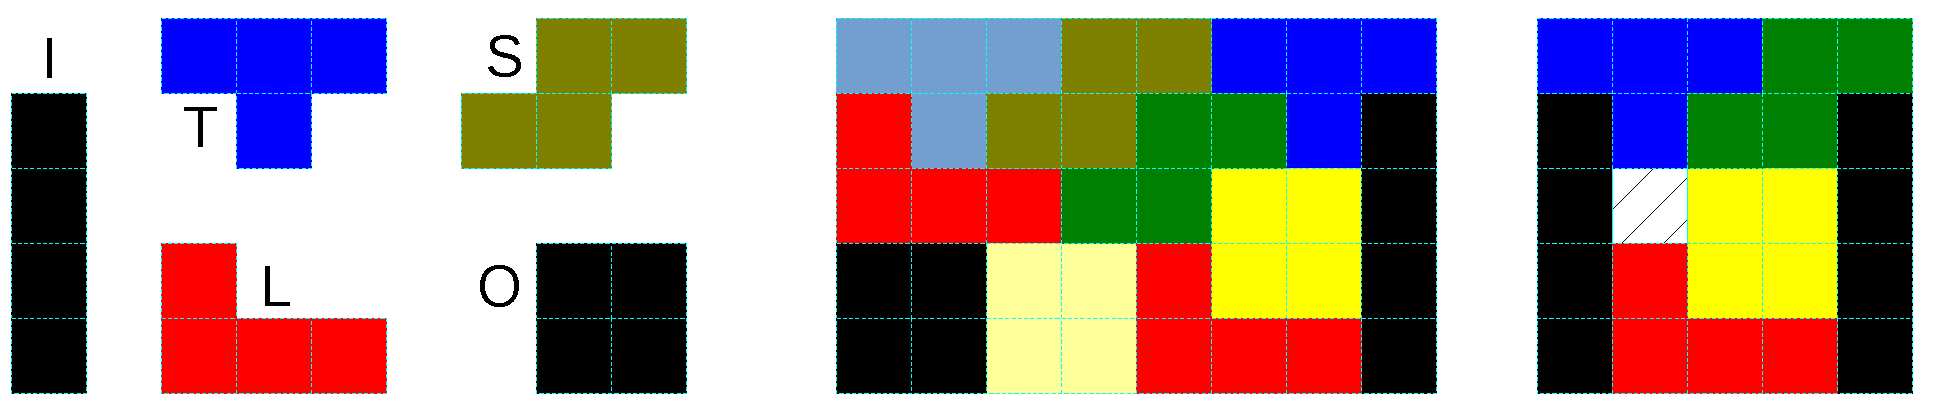
\includegraphics[width=\linewidth]{tetris.pdf}
    \caption{The 5 tetris pieces and two solved puzzles of size 5x8 and 5x5 blocks}
    \label{fig:tetris}
\end{figure}

Figure~\ref{fig:tetris} shows the five types of pieces and two examples.
The left example shows how to arrange one I, two each of T, L, S, and three O pieces into a $5 \times 8$ block.
This is represented by the seven arguments ``5 8 1 2 2 2 3.''
The block doesn't have to be filled completely.
The example on the right shows a solution for the input sequence ``5 5 2 1 1 1 1,'' which is to arrange two I pieces and one of each remaining type in a $5 \times 5$ block, leaving one empty cell.
An example of an unsolvable instance could be ``4 4 1 1 0 1 1.''

\section{Local Search Competition (10 Points)}

The objective is to implement a stochastic local search SAT solver.
Instances that are both easy to solve and satisfiable can be found in GBD.\footnote{\url{https://benchmark-database.de/?minisat1m=yes&result=sat}}
The solvers will be evaluated on a random subset of these instances, as well as on other instances, including a set of random 3-SAT instances and some instances that are unsatisfiable.
The format for the satisfying assignment should be identical to that used in the SAT competition.\footnote{\url{https://satcompetition.github.io/2024/output.html}}


\end{document}